\documentclass[14pt]{extarticle}
\usepackage[english,ukrainian]{babel}
\usepackage[utf8]{inputenc}
\usepackage{amsmath,amssymb}
\usepackage{parskip}
\usepackage{graphicx}
\usepackage{xcolor}
\usepackage{tcolorbox}
\tcbuselibrary{skins}
\usepackage[framemethod=tikz]{mdframed}
\usepackage{chngcntr}
\usepackage{enumitem}
\usepackage{hyperref}
\usepackage{float}
\usepackage{subfig}
\usepackage{esint}
\usepackage[top=2.5cm, left=3cm, right=3cm, bottom=4.0cm]{geometry}
\usepackage[table]{xcolor}
\usepackage{algorithm}
\usepackage{algpseudocode}
\usepackage{listings}

\title{Контрольна робота 2 з курсу ``Дискретна теорія ймовірності''}
\author{Студента групи МП-31 Захарова Дмитра Олеговича}
\date{\today}

\begin{document}

\maketitle

\begin{center}
\textbf{Варіант 3.}
\end{center}

\section*{Завдання.} 

\textbf{Умова.} Випадкова величина $\xi$ приймає значення $0,2,-1,1$ з ймовiрностями $0.1, 0.2, 0.3,a$ вiдповiдно. Знайти значення параметра $a$, функцiю розподiлу випадкової величини $\xi$ та побудувати її графiк. Знайти математичне сподiвання та дисперсiю випадкової величини $\xi$, а також ймовiрностi $\mathbb{P}(0 \leq \xi \leq 2), \mathbb{P}(0<\xi<2)$.

\textbf{Розв'язання.} Позначимо $\mathcal{X} = \{0,2,-1,1\}$ -- набір усіх можливих значень випадкової величини. Щоб дискретний розподіл ймовірностней $\mathbb{P}(\xi=k)$ був коректно визначено, повинно виконуватись
\[
\sum_{x \in \mathcal{X}}\mathbb{P}(\xi=x) = 1
\]
Отже маємо:
\begin{gather*}
\mathbb{P}(\xi=0) + \mathbb{P}(\xi=2) + \mathbb{P}(\xi=-1) + \mathbb{P}(\xi = 1) = 1 \\
\implies 0.1 + 0.2 + 0.3 + a = 1.0 \implies \boxed{a=0.4}
\end{gather*}
Тепер знайдемо функцію розподілу $F_{\xi}(x)$. Якщо ми розташуємо елементи $x_1,x_2,\dots,x_N$ множини $\mathcal{X}$ у зростаючому порядку з відповідними ймовірностями $p_1,\dots,p_N$ (тобто $x_1<x_2<\dots<x_N$), то отримаємо функцію розподілу:
\[
F_{\xi}(x) \triangleq \begin{cases}
    0, & x \leq x_1 \\
    \sum_{i=1}^k p_i, & x_k < x \leq x_{k+1}, \; k \in \{1,\dots,N-1\}\\
    1, & x > x_N
\end{cases}
\]
Отже, підставляємо:
\[
F_{\xi}(x) = \begin{cases}
    0, & x \leq -1 \\
    0.3, & -1 < x \leq 0 \\
    0.4, & 0 < x \leq 1 \\
    0.8, & 1 < x \leq 2 \\
    1.0, & x > 2
\end{cases}
\]

Графік цього розподілу зображено на рис. \ref{fig:1}.
\begin{figure}[H]
    \centering
    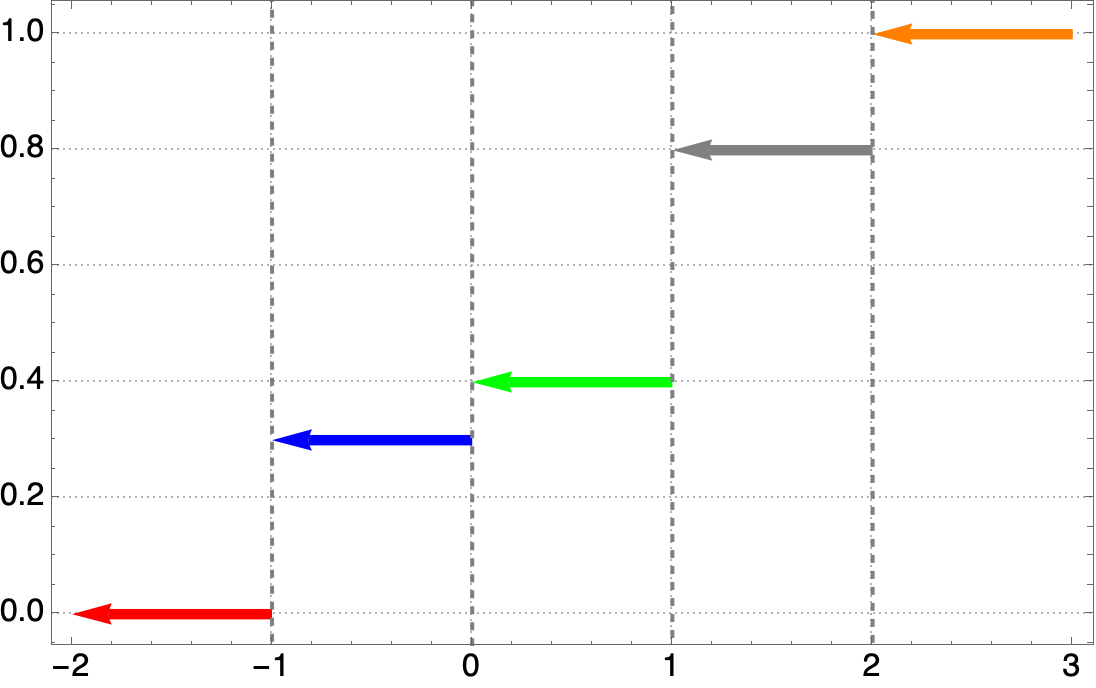
\includegraphics[width=0.7\textwidth]{images/test_2/distribution_plot.png}
    \caption{Графік функції $F_{\xi}$ розподілу випадкової величини $\xi$}
    \label{fig:1}
\end{figure}

Знайдемо математичне сподівання та дисперсію. За означенням, математичне сподівання:
\begin{gather*}
\mathbb{E}[\xi] \triangleq \sum_{x \in \mathcal{X}} x \cdot \mathbb{P}(\xi=x) \\
= 0 \cdot 0.1 + 2 \cdot 0.2 + (-1) \cdot 0.3 + 1 \cdot 0.4 = 0.4-0.3+0.4=0.5
\end{gather*}
Для знаходження дисперсії знайдемо $\mathbb{E}[\xi^2]$. Cкористаємося тим фактом, що $\mathbb{E}[f(\xi)] = \sum_{x \in \mathcal{X}}f(x)\mathbb{P}(\xi=x)$. Тоді
\begin{gather*}
\mathbb{E}[\xi^2] = \sum_{x \in \mathcal{X}} x^2 \cdot \mathbb{P}(\xi=x) 
= 0^2 \cdot 0.1 + 2^2 \cdot 0.2 + (-1)^2 \cdot 0.3 + 1^2 \cdot 0.4 \\
= 0.8 + 0.3 + 0.4 = 1.5
\end{gather*}
Отже, дисперсію можна знайти за формулою
\[
\text{Var}[\xi] = \mathbb{E}[\xi^2]-\mathbb{E}[\xi]^2 = 1.5 - 0.5^2 = 1.25
\]
Нарешті, знайдемо ймовірності з умови. Маємо:
\[
\mathbb{P}(0 \leq \xi \leq 2) = \sum_{x \in \mathcal{X}: 0 \leq x \leq 2}\mathbb{P}(\xi=x) = \mathbb{P}(\xi=0)+\mathbb{P}(\xi=1) + \mathbb{P}(\xi=2)=0.7
\]
\[
\mathbb{P}(0 < \xi < 2) = \sum_{x \in \mathcal{X}: 0 < x < 2} \mathbb{P}(\xi=x) = \mathbb{P}(\xi=1) = 0.4
\]

\textbf{Відповідь.}
\begin{enumerate}
    \item $a=0.4$;
    \item $F_{\xi}$ див. у розв'язанні;
    \item $\mathbb{E}[\xi]=0.5$;
    \item $\text{Var}[\xi]=1.25$;
    \item $\mathbb{P}(0 \leq \xi \leq 2) = 0.7$;
    \item $\mathbb{P}(0 < \xi < 2) = 0.4$.
\end{enumerate}

\end{document}

